% CPE 458
% Dr. Chris Lupo

% Two Column Format
%this allows us to specify sections to be single or multi column so that things
% like title page and table of contents are single column

%multiple citations:
\documentclass[12pt]{article}
\usepackage{multicol}
\usepackage{setspace}
\usepackage{multirow}
\usepackage{enumerate}
\usepackage{url}
\usepackage{framed}
\usepackage{verbatim}
\usepackage{geometry}
\usepackage{changepage}
\usepackage{amsmath}
\usepackage{graphicx}
\usepackage{graphics}
\usepackage{tabularx,array,ragged2e,comment}
%%% PAGE DIMENSIONS
\usepackage{geometry} % to change the page dimensions
\geometry{letterpaper}
\newcommand{\tab}{\hspace*{2em}}

\begin{document}

\setlength{\parindent}{1cm}
\title{\vfill A Practical Approach to Distributed WPA/WPA2 Cracking with CUDA} 

%\vfill gives us the black space at the top of the page

\author{Sunjay Dhama, Cal Poly San Luis Obispo\vspace{12pt} \\
sdhama@calpoly.edu\vspace{12pt} \\
%%Dr. Chris Lupo, Cal Poly San Luis Obispo
%%clupo@calpoly.edu 
}
\date{\today}

\maketitle
\vfill
\begin{abstract}
This project builds upon the work presented by security research Thomas Roth at Defcon 20 by providing a practical implementation to cracking Wi-Fi Protected Access (WPA) and Wi-Fi Protected Access II (WPA2) passwords with Compute Unified Device Architecture (CUDA) \cite{roth}. It does this by incorporating a password database that allows an attacker to easily store their word list in a database, which the cracking nodes query.
This paper describes the implementation of the attack and discusses countermeasures to help mitigate it. 
\end{abstract}
%%%This work expands upon the former by providing a practical implementation to cracking WPA passwords with CUDA by integrating a password database that allows an attacker to store their word list in a database, which the cracking nodes query from. 

\thispagestyle{empty} 
%remove page number from title page
\newpage
%Create a table of contents with all headings of level 3 and above.
%http://en.wikibooks.org/wiki/LaTeX/Document_Structure#Table_of_contents has
%info on customizing the table of contents
\thispagestyle{empty} %Remove page number from TOC
\tableofcontents
\newpage
%Start numbering first page of content as page 1
\setcounter{page}{1}
\section{Introduction}
\indent The first section of this report will go over background information, so the reader can fully comprehend the work presented. The next section will give an overview of related work. The third section will detail why this implementation is important. The fourth section will discuss the technical details of the work. The fifth section will go over results. The sixth section will speak about ways to mitigate this attack. The second to last section will draw some conclusions and the final section will make suggestions for future work.
\section{Background}
\indent This work utilizes three important concepts: WPA, CUDA, and Amazon Web Services (AWS) Elastic Compute Cloud (EC2). Each of these three pieces were integral in this project.
\subsection{WPA}
WPA/WPA2 are security protocols released in 2003 and 2006 for wireless LAN communication, and are meant to provide confidentiality and integrity \cite{ieee} . WPA/WPA2 was designed in order to fix flaws in Wired Equivalent Privacy (WEP) \cite{practical}, which has been shown to be easily exploitable \cite{wep}. Neither WPA nor WPA2 are completely secure anymore either. Researchers Martin Beck and Erik Tews showed how to exploit some of their flaws\cite{tews}. However, their work is beyond the scope of this project, which does not utilize those discovered flaws. Simply put, this project assumes WPA/WPA2, which are essentially a modified version of SHA-1, are unflawed crytographic hashing algorithms.\\
\indent By definition, SHA-1 is a one-way function, which means given the output of a text encoded by SHA-1, the original text cannot be derived without the key\cite{sha1}. However, there are several methods to obtaining a WPA/WPA2 password. The most predominant method is a dictionary-based attack where the attacker uses a word list of possible passwords and the Access Point (AP) name to generate Pairwise Master Keys (PMKs) \cite{cck}. A PMK is used to generate a Private Transient Key (PTK), which is used to generate a Message Identity Code (MIC) \cite{cck}. The generated MIC and the MIC captured by an attacker from the four-way handshake, the process of a computer authenticating itself to the router when attempting to join the network, are then compared to determine if they match \cite{cck}. If there is a match, the password used to generate the PMK is the password for the network \cite{cck}. This is the type of attack examined. \\
\indent When WPA/WPA2 was first developed, it was infeasible to crack a password over 7 characters in length due to amount of time required to generate each PMK \cite{gpu}. However, since the release of the CUDA SDK, which allows programmers to utilize the General-Purpose Computing on Graphics Processing Units (GPGPU) for computationally intense operations other than graphics processing, the feasibility of cracking WPA/WPA2 has increased exponentially \cite{gpu}.

%use later
%Eavesdropping the network, the goal of the attacker is to get a handshake; the hash of the key swapped between the client and the AP when the client begins the connection. The attacker can wait, or launch a de-authenticate the client.
\subsection{CUDA}
\indent
The release of the CUDA SDK drastically changed the landscape of encryption. Roth noted this when he said:
\begin{quotation}
Modern high-end GPUs feature more than 400 cores which can be used to accelerate a lot of applications in the science sector, in the medical sector, in the financial sector and in the \emph{encryption sector} - practically everywhere where the same program needs to run over a large amount of independent data elements.
\end{quotation}
Running the same program ``over a large amount of independent data elements'' is exactly what happens during a dictionary-based attack, so it is logical to incorportate the CUDA SDK \cite{roth}. Leveraging the CUDA SDK to speed up the cracking process has been prevalent for several years and a multitude of other cracking applications exist that utilize it. Three of the most popular applications are Pyrit, oclHashcat, and Cryptohaze Multiforcer \cite{pyrit,ocl,crypto}.\\
\indent However, all three have drawbacks. While oclHashcat is arguably the fastest hash cracking software available to date, it is not open-source and until very recently, did not support running in a distributed environment \cite{ocl1}. The only currently available open-source software to utilize CUDA to crack WPA/WPA2 is Pyrit, which has \textit{limited} support for running in a distributed environment \cite{pyrit}. However, Pyrit is not maintained and has a number of bugs that hamper adoption of it \cite{pyrit}. Cryptohaze Multiforcer is very similar to this project \cite{crypto}. It too supports easily cracking password hashes in a distributed environment, but presently does not support cracking WPA/WPA2 \cite{crypto}. This project seeks to overcome all of those issues by being completely open-source and easy for the non-technical user to run when crack WPA/WPA2 in a distributed environment. However, obtaining access to a large number of physical computers with both Nvidia GPUs and the CUDA SDK installed can be a challenge.
\subsection{AWS EC2}
\indent If a user does not have access to physical computers with Nvidia GPUs, EC2 offers customers the option of paying per hour for the usage of virtual computers, referred to as instances \cite{ec2}. It is no longer necessary to spend thousands of dollars on a \textit{cracking rig} \cite{gosney}. Instead, one pays for the amount of time they need \cite{ec2}. EC2 is of interest in this application due to the introduction of GPU instances, which were used to benchmark this application. They have the following specifications:\\
\begin{table}[htbp]
\begin{center}
\begin{tabular}{ |c|c|c| } % center
 \hline
 \textbf{Cluster GPU Quadruple Extra Large Instance} \\ % LINE1
 \hline
 22 GB of memory\\ % LINE2
 \hline
2 x Intel Xeon X5570, quad-core ”Nehalem” architecture\\% LINE3
 \hline
2 x NVIDIA Tesla ”Fermi” M2050 GPUs\\%LINE4
 \hline
1690 GB of instance storage\\%LINE5
\hline
64-bit platform\\%LINE6
\hline
 I/O Performance: Very High (10 Gigabit Ethernet)\\%LINE7
\hline
API name: cg1.4xlarge \\%LINE8
\hline
 \end{tabular}
\end{center}
\caption{EC2 Instance cg1.4xlarge Specifications}
\end{table}
\\
% The GPU programming was done using CUDA tools version 5.0. 
%It is important to note this application can be run on an EC2 GPU instance or on any physical computer with the CUDA SDK installed. 
%section 1

\section{Existing work}
\indent Before going into detail about this project, it is necessary to summarize previous work. Although Roth has not publically released the source code for his application, others following the steps he laid out did \cite{cck}. In 2012, Chaodong Zheng, Chengwen Luo, and Kartik Sankaran (ZLS) from the University of Singapore released their implementation of Roth's code, which is continued by this project \cite{cck}.
\subsection{Importance}
ZLS's work was important for the following reasons:
\begin{enumerate}[(I)]
\item ZLS removed almost all monetary barriers to entry into advanced password cracking \cite{cck}. Essentially anyone could partition EC2 GPU instances and crack passwords \cite{cck}.
\item The rate at which it takes for the password to be found decreases linearly with additional EC2 instances. An attacker with a high value target could launch more instances and generate more PMKs per second \cite{cck}.
\end{enumerate}
\subsection{Summary}
Since this application built upon ZLS's source code, it is necessary to explain what they did and their results. However, the most benefit can be gained from reading their work in full. ZLS leveraged the AWS API to create a program that automates the creation of EC2 GPU instances to crack WPA/WPA2 passwords \cite{cck}. The master program relays the needed information to two (or more) GPU instances and those instances iterate through their range of passwords \cite{cck}. Their work made use of the open-source implementation of WPA/WPA2, which can be found in Pyrit \cite{cck,pyrit}. They were able to achieve a cracking efficiency of 25,000 PMKs/s/dollar by using spot instance pricing, which is an improvement over Roth, who achieved 22,500 PMKs/s/dollar \cite{cck,roth}.

\section{Motivation}
\indent The primary motivation for this work was to give security penetration testers (pentesters) a tool they could use when auditing large companies. Pentesters typically have varying degrees of experience with programming and often utilize software tools to aid in their audit. Pentesters want tools that are effective and easy to use. To do this, ZLS's code had to be modified.
\subsection{Practicality}
\indent This work is important because the publically released source code of ZLS does not provide a practical implementation for cracking WPA/WPA2 as ZLS's application checks only phone numbers when attempting to crack a password. Although use of one's phone number as one's router password is a popular choice among consumers, it is not all-encompassing \cite{cck}. In personal experimentation and surveying of peers, it was found that phone numbers accounted for a user's password roughly 20\% of the time. This means that 80\% of the time, the password could not be found due to it not being a phone number. However for several years, crackers have been using large \emph{cracking dictionaries}, files with a large list of words that are commonly used as passwords, in an attempt to check \textit{only} the most common passwords. Dictionary-based attacks continue to be used to crack passwords because they are still effective \cite{practical}. 
\indent This work took the concept of the word list and simply put it online in a database. This means an attacker is no longer limited to phone numbers, but only by how comprehensive their word list is. However, an attacker is never truly limited by the number of words in their word list as more comprehensive dictionaries are released on a regular basis and better ones can always be generated \cite{dict}. 
%My work only tested password 8 to 12 characters in length simply because in my experience most user passwords are that length.
% but with this work, I hope it will increase to a point where it would become infeasible to crack.
\subsection{Ease of Use}
\indent Although not the focus of this work, the pcap2hccap software was expanded upon \cite{cap}. The added functionality allows a user to specify a packet capture containing the four-way handshake and generate the .txt file, which is needed by this application to crack a given AP password. It was not immediately clear how ZLS originally generated their .txt file, but with the additions made to the pcap2hccap program, the process is now trivial. This removed another barrier to entry to cracking WPA/WPA2 passwords. \\
\indent Another area in which was not the focus of this work, but which was made easier through automation was the creation of the database. A C++ program with a command-line interface creates the database and inserts words from a user specified file for the user. The user needs only a basic understanding of Database Management Systems (DBMSs) to generate the word list database.\\
\indent Increasing ease of use and implementing a practical attack were main motivations for this project. If more users are able to crack router passwords easily, people will think twice about using a simple or default password and hopefully use a randomly generated one. Software such as LastPass can facilitate that\cite{last}. 


%section 2


\section{System Architecture}
As shown in Figure 1, the entire system includes one master node, multiple slave nodes, and one word list database. The master node runs the master program, the slave nodes run the cracking program, and the database node runs a MySQL database, which is opento the slave nodes for connection. The user specifies the location of the handshake file, which they have generated using the modified pcap2hccap application, the number of slave nodes, the port number at which those slave nodes are expecting a connection, the IP addresses of the slave nodes, the IP address of the database, and the range of passwords in the database that the user would like to check. The user puts all of the aforementioned information into a configuration file, which the master program reads and uses to distributes the work to the running slave nodes. Once the slave nodes recieve the necessary information from the master node, they begin querying the database for their range of passwords and generating PMKs. Once the PMKs are generated, the slave nodes generate the MICs and compare them against the existing MIC. If there is a match, the slave will send the password back to the master. The master will then tell the other slave nodes to stop running. If there is not a match, the slaves will request more passwords from the database and the process will continue until either the password is found or there are no more passwords to query for in the range.
\begin{figure}[htbp]
\begin{center}
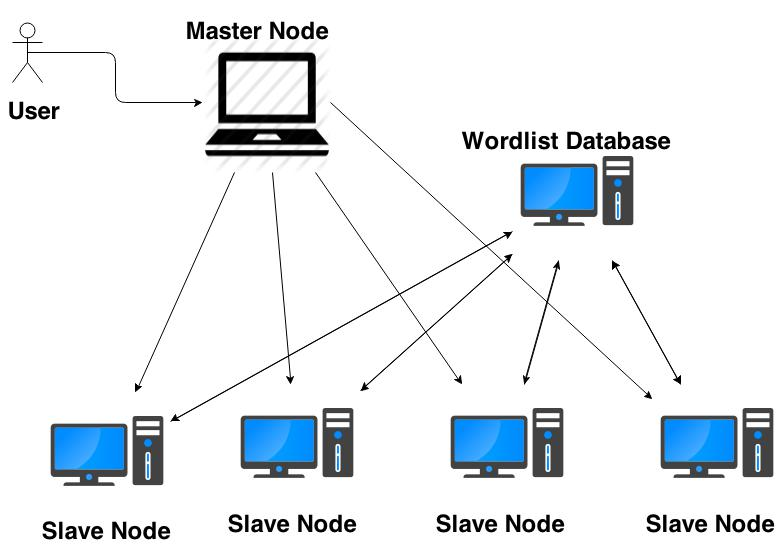
\includegraphics[width=120mm]{Senior_Project.jpg}
\end{center}
\caption{System Architecture}
\label{overflow}
\end{figure}
\section{Implementation}
The implementation of this project has 3 main parts, the master node, the slave node(s), and the database. The master node provides a way for the user to interact with the program. The cracking program has two distinct parts, the CPU code and the GPU code, both of which were modified. The final piece was the database code, which did not require a lot of programming, but moreso a lot of setup.
\subsection{Master}
\indent The original implementation of the master node was fairly simplistic. It simply created the AWS instances using the API, sent all the instances the necessary information for cracking and then waited. During this waiting period, it did no computation. It simply checked if the slaves have sent back the password. It seemed wasteful to create an AWS instance to do this, so the code was modified to run on the local machine. \\
\indent There was only one one main piece of functionality added to the master code. It was to  remove the limitation that the slave nodes be only AWS instances. Instead, a configuration file where a user can specify the information required by the application, was added. This means that if a user has access to a large number of PCs either at home or at work, those could be utilized as well. No modifications were made to the original code that launched the EC2 GPU instances. That file was simply excluded. In all but the last testing phase, testing was done on either local or university machines. This not only saved money, but also was easier overall.\\
\indent It is important to point out that in the original implementation it was not possible for the master program to launch an instance and have it run the cracking program. One needed to have already installed the CUDA SDK and necessary dependencies on the instance and then compile and run the slave code. Once a user had done that, they could create a snapshot of the instance and use the program to load that image onto the instance, so it would be ready to connect to the master program. This process is too technically long and complex for the a user and too time-consuming for any pentester. Most pentesters would either a) Already have several physical or virtual machines at their disposal to run the cracking code on or b) Would not bother with creating a snapshot of a configured instance, but simply create and configure the instances manually as needed. This is why there is an easy to use script incorporated into this project to help in the configuration process of an EC2 GPU instance.
\subsection{Slave}
\indent There were many areas for improvement in the original implementation, but the focus was on making this tool practical. This is why the main modification to the cracking code was the incorporation of reading passwords from a MySQL database. Once it became clear the original implementation for dividing the password range between the CPU and GPU threads would still work, it was just a case of using those ranges when querying from the database. Due to the fact that the greatest number of open connections to the database from one particular instance would not exceed 30 (highly unlikely a single PC would have more than 30 CPU threads and GPUs combined), a connection pool was not utilized. Each CPU thread has its own connection to the database and makes queries independent of the other threads, so the threads do not have to wait for each other. Each CPU thread queries for a set number of passwords, known as the CPU Password Size. The passwords are then individually passed to a function, which generates the PMKs and MICs. The GPU code is not much different except the number of passwords it queries for is far greater and is referred to as the GPU Password size. As one would expect, the GPU code does all the generation of the PMKs on the GPU and then transfers the result back to the CPU to generate and compare the MICs.\\
\indent After profiling the CUDA portion of the cracking code, the limiting factor for the total number of threads present in each CUDA kernel was registers. An attempted solution to this was to break the kernel into two kernels and call them one after another. The first kernel computed the first 4096 iterations of SHA-1 and the second kernel computed the second 4096 iterations. Unfortunately, this did not provide any speedup. In fact, there was a slow down of about 10\% in the number of PMKs generated per second, but there was not time to investigate further. It is likely that the overhead of calling the kernel multiple times removes any benefit of additional registers.
% The main thing I would do differently if I had more time would be to query the database less frequently and simply put the most number of passwords into global GPU memory at the very beginning. A final important thing to note is that the code is not fully tested with multiple graphics cards, simply because it is expensive to run the CG1 instance and I did not have access to any other machines with multiple GPUs. 
\subsection{Database}
\indent In thinking about how to make ZLS's code more practical, it was clear a word list had to be added, but how best to implement it is the challenge After much thought, a MySQL database, hosted on an AWS instance, was used. This would allow a large number of slaves to connect to the database at one time with no lag. A MySQL database was chosen because MySQL is billed as a \emph{production level} database, used by many commercial enterprises. To ease in the setup of the database, a C++ application was developed, which not only created the database, but also quickly inserts the potential passwords from a file up to 1GB in size. There was much internal debate about how best to load and store a file, but in the end an in-memory database had too many drawbacks. The main drawback with an in-memory database is not only the potential for corruption, but also that the size of the database could be grow to be greater in size than that of memory. So, a MySQL database was launched on an EC2 instance with the following specifications:\\
%and spent a lot of time trying to integrate the function mmap, a fast way to read a file into memory as  a way to store the wordlist in memory. 
\begin{table}[htbp]
\begin{center}
\begin{tabular}{ |c|c|c| } % center
 \hline
 \textbf{Cluster CPU Quadruple Extra Large Instance} \\ % LINE1
 \hline
 23GB of 1333MHz DDR3 Registered ECC memory\\ % LINE2
 \hline
2 x Intel Xeon X5570   (quad-core Nehalem)\\% LINE3
 \hline
2 x 845GB 7200RPM HDDs\\
\hline
64-bit platform\\
\hline
 I/O Performance: Very High (10 Gigabit Ethernet)\\
\hline
API name: cc1.4xlarge\\
\hline
 \end{tabular}
\end{center}
\caption{EC2 Instance cc1.4xlarge Specifications}
\end{table}
\\
\section{Results}
\indent Although this project is still a work-in-progress, some great things were achieved. The most obvious result is that users now have the ability to easily run this cracking software on physical hardware as well as virtual using words from their own word lists. There is the added barrier of creating a database, but unless the word list is split up and placed on each machine, there is no other way to easily overcome this obstacle.
%\newpage
\subsection{Benchmarks}
\indent The benchmarks shown in Table 3 were achieved with the password located at index 5,555,555. However, due to the GPU Password Size more PMKs than necessary were always generated.
\begin{table}[htbp]
\centering
%%%\begin{adjustwidth}{-1cm}{}
\begin{tabular}{ |c|c|c|c|c|c|}  % center
 \hline
 CPU Password Size & GPU Password Size &  Passwords Tested & Time (s) & PMKs/s\\ % LINE1
 \hline
 0 & 100,000 & 5,600,000 & 202 & 27,722  \\ % LINE2
 \hline
 0 & 500,000 & 6,000,000 & 186 & 32,258 \\ % LINE3
 \hline
 0 & 1,000,000 & 6,000,000 & 183 & 32,786 \\ % LINE3
 \hline
 0 & 2,000,000 & 8,000,000 & 236 & 33,898 \\ % LINE3
 \hline
 50,000 (8 threads) & 1,000,000 & 6,000,000 & 222 & 27,027 \\ % LINE3
\hline
 100,000 (8 threads) & 500,000 & 5,800,000 & 207 & 28,019  \\ % LINE3
\hline
 100,000 (16 threads) & 500,000 & 6,100,000 & 248 & 24,596  \\ % LINE3
\hline
 \end{tabular}
\caption{Benchmarks}
\end{table}
As the reader can see, having 0 CPU threads increased the overall speed. This is likely due the fact that each thread has its own database connection, which slowed things down. Additionally the number of PMKs/s increased as the GPU Password Size increased, meaning there was a fair amount of overhead associated with transferring data on and off the GPU. The fastest recorded speed was 33,898 PMKs per second.  Unfortunately, this is substantially less than the roughly 48,000 PMKs/s that Roth achieved \cite{roth}. However, with some more optimizations that speed could be obtained.
%Future work would be to query for a million passwords then let the GPU do the rest. It does not make sense for each thread to have its own MySQL connection. There should have only been two MySQL Connections. One for the CPU and one for the GPU. They would both get a lot of passwords in the very beginning and store in memory and then distribute. The fastest time was when least number of queries done, which is why whenever any amount of CPU threads were added the PMKs/sec went down as the overhead of a query is large, so large that a CPU thread is negligible.


%third to last
\section{Mitigation Techniques}
\indent This work is proof that both WPA and WPA2 are not secure protocols and should be avoid whenever possible. Unfortunately, the highest grade encryption offered by some consumer-grade routers is WPA2. If that is the case and a more secure algorithm cannot be chosen, the best option is to use a passphrase longer than 12 characters that is randomly generated and contains both uppercase and lowercase letters as well as symbols. This ensures that the password does not exist in any cracking dictionary. The password to the network should also be changed every 6 months and whenever a guest has finished using the network. Another preventative measure is to limit the signal range of one's router to only areas a user controls, in order to prevent an attacker from obtaining a four-way handshake. Without the handshake, an attacker cannot penetrate the network \cite{cck}. A final precaution would be to use a Virtual Private Network (VPN) while at home, so that even if an attacker does gain access to the network, s/he cannot access any of the information being sent or receive as it is encrypted. However, this is not guaranteed \cite{moxie}.

%I wish I had spent more time investigating previous work in this field as there is far more than I expected and it could have helped me avoid some of the roadblocks I ran into.

%Second to last
\section{Conclusions}
\indent With the introduction of the cloud and applications that easily distribute work, combined with the speedup achieved by leveraging CUDA, use of WPA/WPA2 for any secure transactions is no longer acceptable. Unless router manufactures switch to a more secure encryption algorithm, attackers will continue to target WPA/WPA2 due to its known weaknesses \cite{cck}. It does not matter how good one's security procedures and protections are in the corporate environment as attackers will continue to target the point of least resistance, which is the home network. Once an attacker has access to an employee’s home network, it is substantially easier to then gain access to the corporate network. This software aims to increase the effectiveness and success rate of penetration testers, which will help lead to a safer and more secure Internet. 

%Final section
\section{Future Work}
\indent Looking toward the future, there are a number of things yet to be added to this application. The following is a prioritized list of what still needs to be done:
\begin{enumerate}
%%[(I)] if we want roman numerals
\item Limit all CPU and GPU threads to only one database connection each.
\item Query the database for the largest number of passwords possible to store in memory, minimizing the number of queries to the database.
\item Further optimize the CUDA code using with the Nvidia Visual Profiler
%\item Optimize the database queries, so they take as little time as possible
\item Add support for the addition of slave nodes during the cracking process.
\item Support reading from a local or in-memory database.
\item Incorportate this project into the Cryptohaze Multiforcer framework.
\end{enumerate}

\newpage

%cite all the references from the bibtex you haven't explicitly cited
\nocite{*}

\bibliographystyle{IEEEannot}


\bibliography{Bib}
\end{document}



